\section{Proposed Approach}
\label{sec:proposed_approach}

We propose a simple yet highly effective pipeline, AirRoom, for room reidentification that leverages multi-level object-oriented information, as shown in \fref{fig:pipeline}. We will now systematically introduce each module of the pipeline, following the sequence of stages in which they are executed.

\subsection{Global Stage}

In this stage, we utilize the Global Feature Extractor to capture global context features, which are derived from the collective presence of objects within the room. These features are then used for Global Retrieval, coarsely selecting semantically similar candidate rooms from the database.

\subsubsection{Global Feature Extractor}
\label{sec:section3.1.1}

Indoor rooms exhibit fewer variations compared to outdoor environments. They lack diverse topographies, such as aerial, subterranean, or underwater features, and do not experience temporal changes like day-night or seasonal variations. Consequently, collecting large datasets for each indoor room is challenging, complicating large-scale training as seen in many VPR methods \cite{arandjelović2016netvladcnnarchitectureweakly, hausler2021patchnetvladmultiscalefusionlocallyglobal, alibey2023mixvprfeaturemixingvisual}. 

However, indoor rooms are inherently rich in objects, each contributing to the room’s overall semantic context. By leveraging this global context information, we can refine the reference search to specifically focus on rooms with similar semantic features to those in the query image. For this purpose, we prefer backbones pretrained on large image datasets, as they provide strong generalizability and effectively capture informative global context features \cite{kornblith2019betterimagenetmodelstransfer}. Our model selections, therefore, include pretrained CNN-based models such as ResNet \cite{he2015deepresiduallearningimage} and transformer-based self-supervised models like DINOv2 \cite{oquab2024dinov2learningrobustvisual}.

\subsubsection{Global Retrieval}

Using the Global Feature Extractor, we extract global context features for \(M\) query and \(N\) reference images. Let \(\mathbf{Q} \in \mathbb{R}^{M \times D_g}\) and \(\mathbf{R} \in \mathbb{R}^{N \times D_g}\) denote the query and reference features, respectively, where \(D_g\) is the feature dimension. The cosine similarity matrix \(\mathbf{S}\) is then computed as:
% Using the Global Feature Extractor, we first extract global context features for \(M\) query and \(N\) reference images. Given \(M\) query features \(\mathbf{Q} \in \mathbb{R}^{M \times D_g}\) and \(N\) reference features \(\mathbf{R} \in \mathbb{R}^{N \times D_g}\), where \(D_g\) denotes the global context feature dimension, we have a cosine similarity matrix \(\mathbf{S}\):
\begin{equation}
    \mathbf{S}_{ij} = \frac{\mathbf{Q}_i \cdot \mathbf{R}_j}{\|\mathbf{Q}_i\| \|\mathbf{R}_j\|}.
    \label{eq:global feature cosine similarity}
\end{equation}
For each query, we select the top-5 most similar reference candidates using the following formula:
\begin{equation}
    \text{Top}_5(\mathbf{S}_{i, :}) = \text{argsort}(-\mathbf{S}_{i, :})[:5],
    \label{eq:global retrieval}
\end{equation}
where \(\mathbf{S}_{i, :}\) represents the cosine similarity for the \(i\)-th query.

\subsection{Local Stage}

Global context features provide valuable semantic information that helps narrow down the candidate list. However, when faced with many semantically similar rooms, relying solely on global context is insufficient, and local features become increasingly essential. In this stage, we adopt a local perspective by first applying instance segmentation and the Receptive Field Expander to identify objects and patches. We then use the Object Feature Extractor to extract features from both objects and patches, followed by Object-Aware Scoring to further refine the candidate list.

\subsubsection{Instance Segmentation}

For each query image and its corresponding five candidates, we employ instance segmentation methods, such as Mask R-CNN \cite{he2018maskrcnn} and Semantic-SAM \cite{li2023semanticsamsegmentrecognizegranularity}, to identify and delineate individual objects. This process generates each object's mask and bounding box. Next, we calculate the center point \(c\) of each object using its bounding box, as shown below:

\begin{equation}
    c = (\frac{x+W}{2}, \frac{y+H}{2}).
    \label{eq:center point}
\end{equation}
In this equation, \(x\) and \(y\) represent the pixel coordinates of the top-left corner of the bounding box, while \(W\) and \(H\) denote the width and height of the bounding box, respectively.

\subsubsection{Receptive Field Expander}

Single object information alone is not sufficiently discriminative. For example, although different desks may have distinct appearances, they can be found in both dining halls and offices. However, when an object is connected with its neighboring items—such as a desk alongside a computer, keyboard, or notebook—it suggests that the room is more likely to be an office rather than a dining hall. This insight motivates us to expand the receptive field from a single object to a patch containing multiple objects.

Given the center points of all objects in an image, we employ Delaunay triangulation \cite{10.5555/1370949} to generate a triangulated graph of object relationships. Specifically, Delaunay triangulation is applied to the set of object centers, ensuring that no object centers are inside the circumcircle of any triangle. This method maximizes the minimum angle of the triangles, preventing narrow, elongated triangles and ensuring more uniform object adjacency. By analyzing the adjacency relationships among the resulting triangles, we can construct the object adjacency matrix, which encodes the spatial and relational proximity of objects within the room.

\vspace{-10pt}
\begin{figure}[ht]
    \centering
    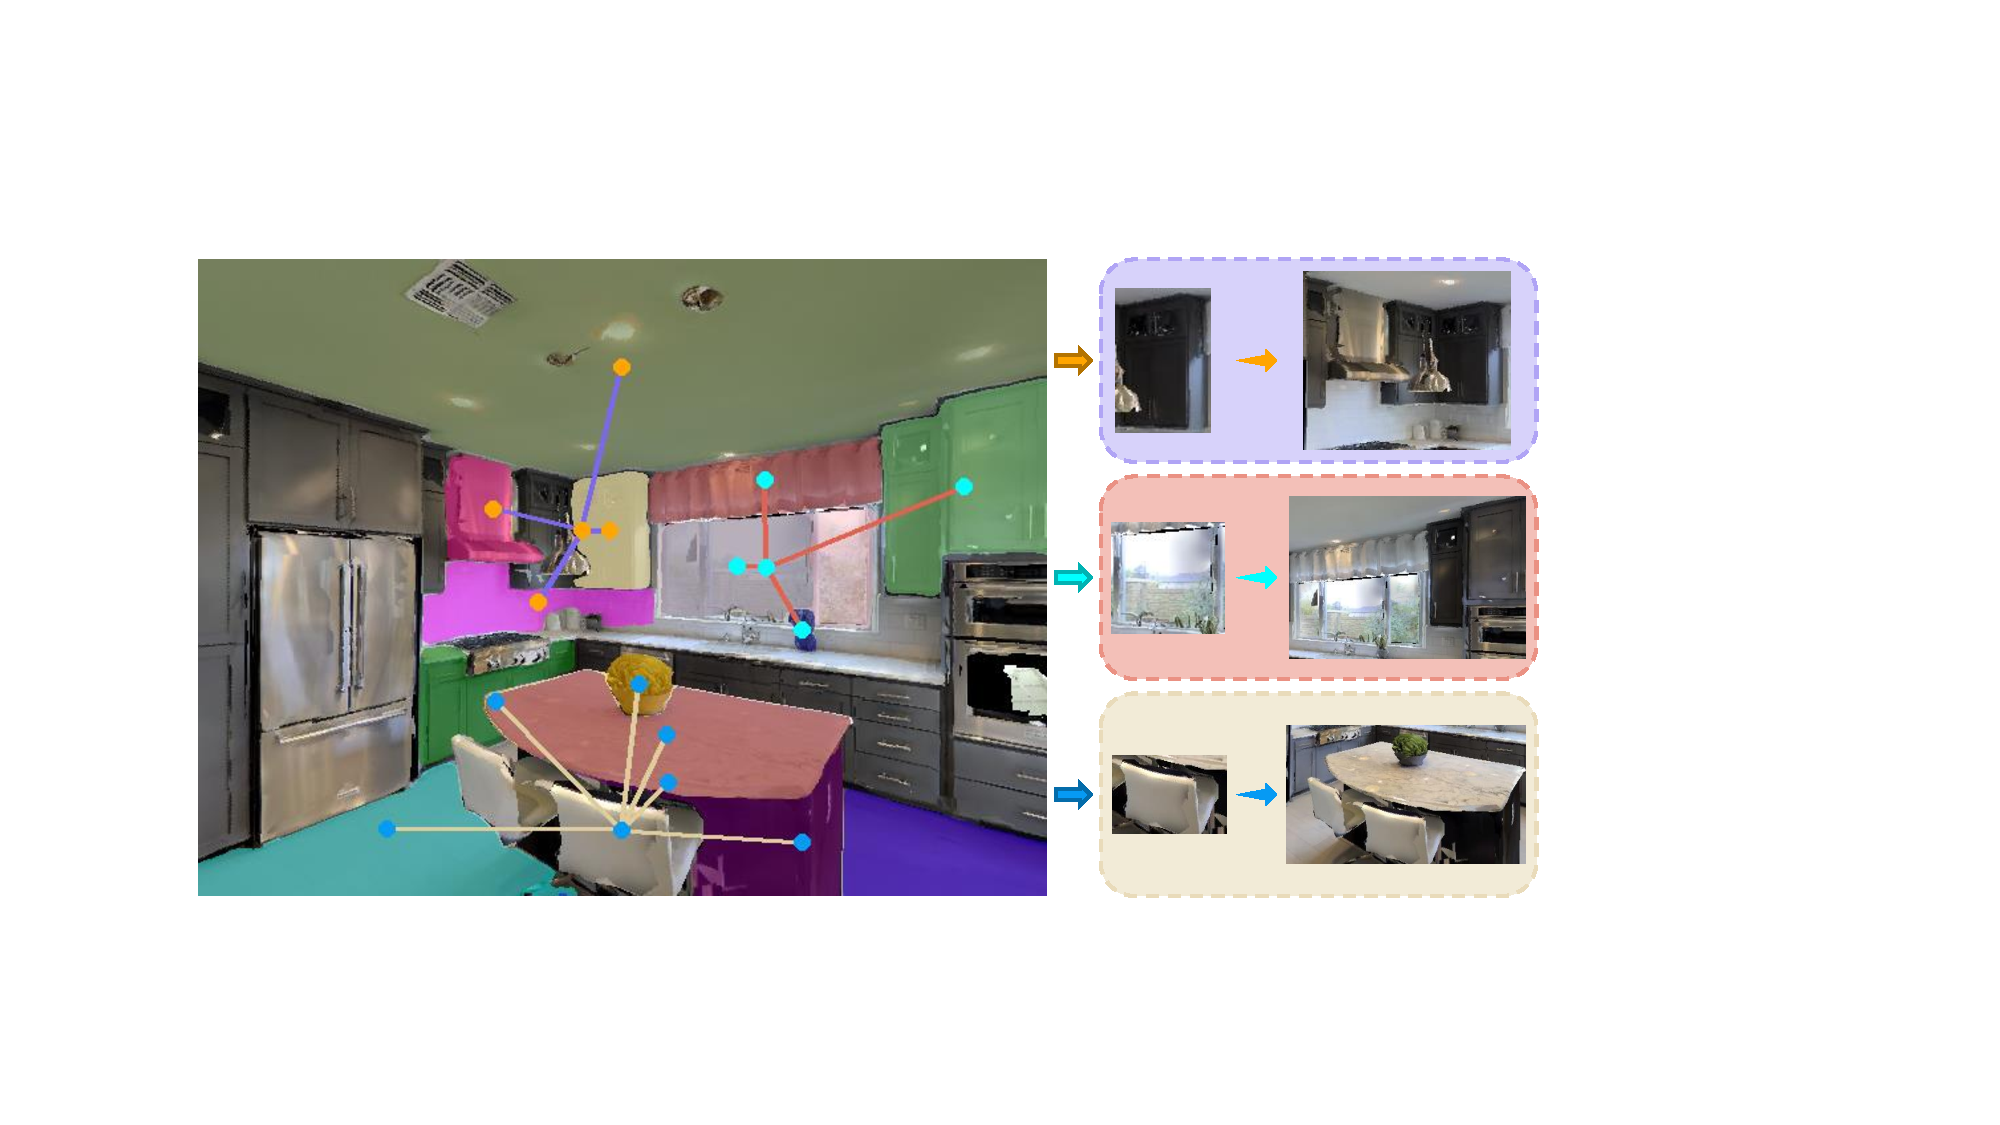
\includegraphics[width=\columnwidth]{expander.pdf}
    \vspace{-20pt}
    \caption{The Receptive Field Expander broadens the receptive field from individual objects to patches rich in contextual information. Leveraging the object adjacency matrix and each object's bounding box, it expands single objects such as a cupboard, window pane, and chair into object patches like a modular kitchen, multi-pane window, and dining set, respectively.}
    \vspace{-5pt}
    \label{fig:expander_image}
\end{figure}

% Given the center points of all objects in an image, we use Delaunay triangulation to create the object adjacency matrix. This mathematical technique takes a set of discrete points and generates triangles that maximize the minimum angle of each triangle, thus avoiding narrow shapes. A key property of Delaunay triangulation is that no discrete point lies within the circumcircle of any triangle formed in the process. By analyzing the adjacency relationships of the triangles created through Delaunay triangulation, we can construct the object adjacency matrix.

Given the object adjacency matrix and bounding boxes in an image, for each object, we consider the bounding boxes of its neighboring objects and enlarge the current object's bounding box to encompass all adjacent objects. This expansion increases the receptive field, enabling us to capture richer contextual information, as illustrated in \fref{fig:expander_image}. We then apply Non-Maximum Suppression (NMS) to select the highest confidence bounding boxes, removing overlapping ones based on their Intersection over Union (IoU) scores. This results in a set of clean, informative object patches.

\begin{figure*}[t]
    \centering
    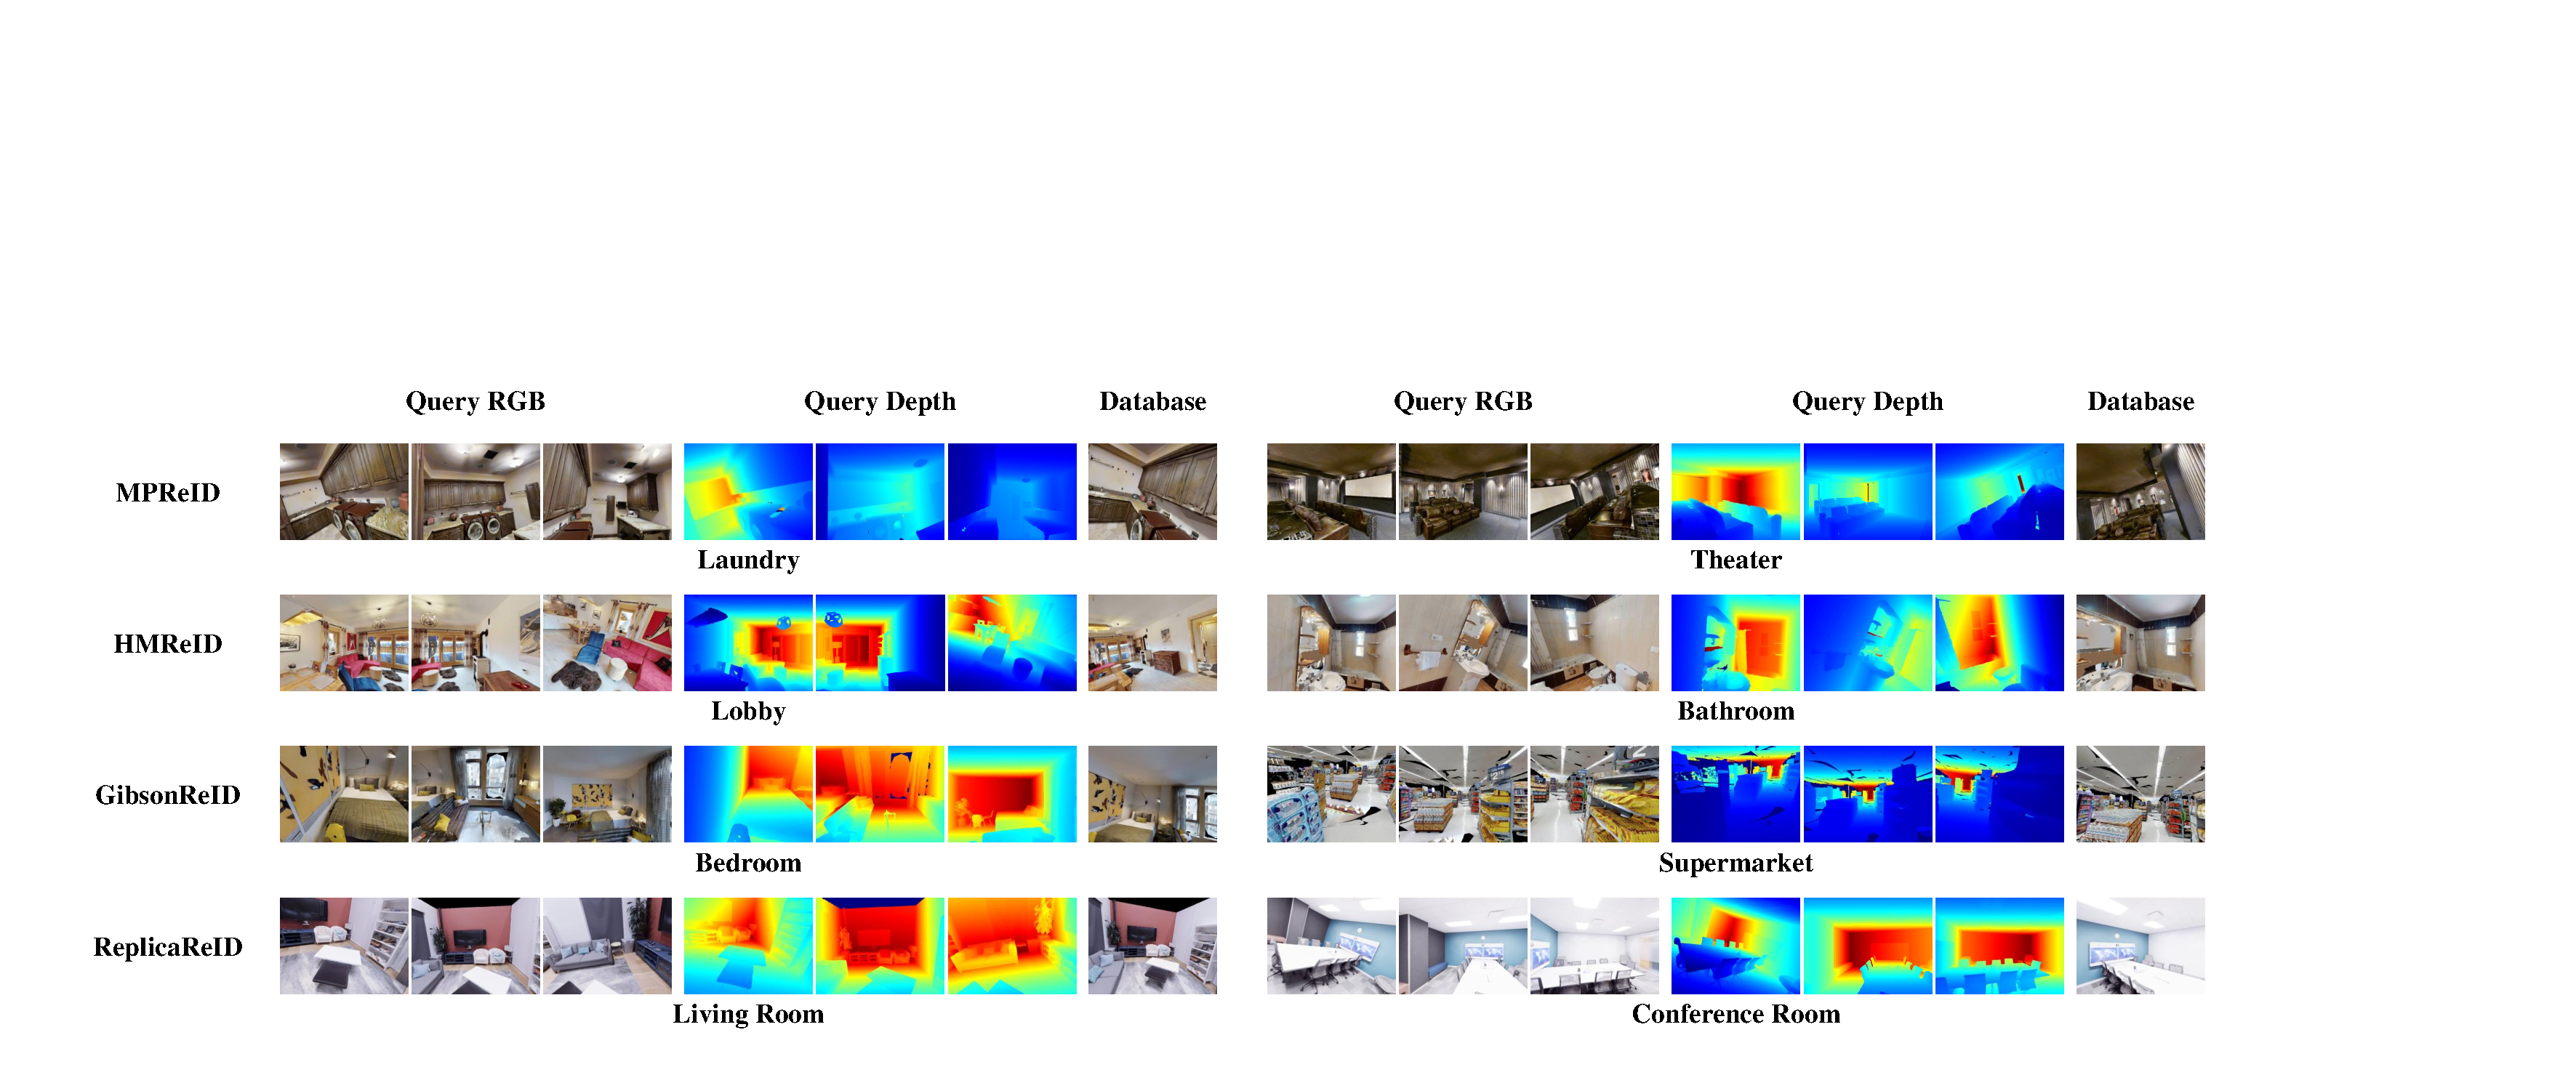
\includegraphics[width=\textwidth]{dataset_font.pdf}
    \vspace{-20pt}
    \caption{Illustration of four newly constructed room reidentification datasets: MPReID, HMReID, GibsonReID, and ReplicaReID. Each room provides only one reference image in the database, while query images for each room capture varied viewpoints.}
    \vspace{-10pt}
    \label{fig:dataset_image}
\end{figure*}

\subsubsection{Object-Aware Refinement}
\label{subsec:refinement}

The Object-Aware Refinement module is composed of three key submodules: Object Feature Extractor, Mutual Nearest Neighbors, and Object-Aware Scoring.

\vspace{-6pt}
\paragraph{Object Feature Extractor}

To effectively leverage object patches and object segmentation information, we prioritize global features over local feature aggregation. The latter approach may fail to capture object characteristics effectively and can significantly increase computational complexity and storage demands \cite{zheng2018sift}. As discussed in Section~\ref{sec:section3.1.1}, we continue to rely on models pre-trained on large image datasets. Using the Object Feature Extractor, we obtain features for both query and reference patches and objects. Let \(Q_p=\{\mathbf{p_i^q}\}_{i=1}^{n_{qp}}\) and \(Q_o=\{\mathbf{o_i^q}\}_{i=1}^{n_{qo}}\) represent the query patch and object feature sets, respectively. For each reference image among the query’s five \mbox{candidates}, we define the reference patch and object feature sets as \(R_p=\{\mathbf{p_i^r}\}_{i=1}^{n_{rp}}\) and \(R_o=\{\mathbf{o_i^r}\}_{i=1}^{n_{ro}}\).

\vspace{-6pt}
\paragraph{Mutual Nearest Neighbors} Given a set of query features \(\{\mathbf{f_i^q}\}_{i=1}^{n_q}\) and reference features \(\{\mathbf{f_i^r}\}_{i=1}^{n_r}\), we obtain feature pairs by identifying mutual nearest neighbor matches through exhaustive comparison of the two sets. Let \(P\) denote the set of cosine similarity scores for these mutual nearest neighbor matches, then we have
\begin{equation}
    P = \{\cos(\mathbf{f_i^q}, \mathbf{f_j^r}) \mid i = \text{NN}_r(\mathbf{f_j^r}), \; j = \text{NN}_q(\mathbf{f_i^q})\}
    \label{eq:mutual nearest neighbors}
\end{equation}
where
\begin{equation}
    \text{NN}_q(\mathbf{f_i^q}) = \arg\max_{j} \left( \frac{\mathbf{f_i^q} \cdot \mathbf{f_j^r}}{\|\mathbf{f_i^q}\| \|\mathbf{f_j^r}\|} \right),
\end{equation}
\begin{equation}
    \text{NN}_r(\mathbf{f_i^r}) = \arg\max_{j} \left( \frac{\mathbf{f_i^r} \cdot \mathbf{f_j^q}}{\|\mathbf{f_i^r}\| \|\mathbf{f_j^q}\|} \right),
\end{equation}
\begin{equation}
    \cos(\mathbf{f_i^q}, \mathbf{f_j^r}) = \frac{\mathbf{f_i^q} \cdot \mathbf{f_j^r}}{\|\mathbf{f_i^q}\| \|\mathbf{f_j^r}\|}.
\end{equation}
% By utilizing mutual nearest neighbors, we can improve retrieval accuracy while narrowing the search space and enhancing retrieval efficiency \cite{zhong2017reranking}.
By utilizing mutual nearest neighbors, we can significantly improve retrieval accuracy, simultaneously narrowing the search space and enhancing overall retrieval efficiency \cite{zhong2017reranking}.

\vspace{-6pt}
\paragraph{Object-Aware Scoring} The object-aware score \(s\) is the sum of the global score \(s_{\text{global}}\) (calculated in Equation~\ref{eq:global feature cosine similarity}), the patch score \(s_{\text{patch}}\), and the object score \(s_{\text{object}}\):
\begin{equation}
    s = s_{\text{global}} + s_{\text{patch}}(Q_p, R_p) + s_{\text{object}}(Q_o, R_o).
    \label{eq:object-aware scoring}
\end{equation}
Here, \(s_{\text{patch}}\) and \(s_{\text{object}}\) can either be \(s_{\text{mean}}\) or \(s_{\max}\), where
\begin{subequations}
\begin{align}
    s_{\text{mean}}(Q_t, R_t) &= \frac{1}{|P(Q_t, R_t)|} \sum_{x \in P(Q_t, R_t)} x,
    \label{eq:mean}\\
    s_{\max}(Q_t, R_t) &= \max_{x \in P(Q_t, R_t)} x.
    \label{eq:max}
\end{align}
\end{subequations}
In these equations, \(P\) denotes the set of cosine similarity scores for mutual nearest neighbor matches, with \(Q_t\) representing either \(Q_p\) or \(Q_o\), and \(R_t\) representing either \(R_p\) or \(R_o\). The global score \(s_{\text{global}}\) serves as a prior, indicating that the initial five candidates vary in relevance. Thus, we retain this term to account for their differing levels of relevance.

\vspace{-8pt}
\paragraph{Object-Aware Refinement} For each query, we select the top-2 most similar reference candidates from the initial five using the Object-Aware Scoring:
\begin{equation}
    \text{Top}_2(\mathbf{s}_{i}) = \text{argsort}(-\mathbf{s}_{i})[:2],
\end{equation}
where \(\mathbf{s}_{i}\) is the object-aware scores for the \(i\)-th query.

\subsection{Fine-Grained Stage}

Patch and object features provide valuable information for understanding the room layout; however, they may be insufficient when distinguishing highly visually similar rooms, particularly in the presence of viewpoint variations and occlusions. Keypoints on objects, by contrast, exhibit strong robustness to texture and appearance variations, enabling them to effectively handle partial occlusions and reject outliers \cite{1498756}. This allows keypoints to offer a more refined approach, capturing finer details for more accurate room identification. In this stage, we use Fine-Grained Retrieval to select the final top-1 result.

\subsubsection{Fine-Grained Retrieval}

Deep matchers, such as SuperGlue \cite{sarlin2020supergluelearningfeaturematching}, perform well in visual localization tasks under challenging conditions, both indoors and outdoors. However, they tend to face efficiency issues. In contrast, LightGlue \cite{lindenberger2023lightgluelocalfeaturematching} offers high efficiency without compromising matching accuracy, making it an ideal choice for our Fine-Grained Retrieval.

For each query image and its two candidate reference images, we match the query to each candidate and record the number of matching keypoint pairs. A higher number of matches typically indicates greater overlap and consistency between the features of the two images, suggesting a higher degree of similarity in their content \cite{Lowe2004DistinctiveIF}. The candidate with more matches is selected as the final result.
